% Please make sure you insert your
% data according to the instructions in PoSauthmanual.pdf
\documentclass[a4paper,11pt]{article}
\usepackage{pos}
\usepackage{xcolor}
\usepackage{subcaption} % Modern package for subfigures
\usepackage{graphicx}   % Required for inserting images
\usepackage{float}
\usepackage{bbm}
\newcommand{\dd}{\mathrm{d}}
\newcommand{\wtil}[1]{\widetilde{#1}}
\newcommand{\deint}[2]{\dd^{#1}\;\!\!#2\;}
\newcommand{\br}[1]{\left\langle #1 \right |}
\newcommand{\kt}[1]{\left| #1 \right \rangle}
%
\newcommand{\Ntot}{N_{\mathrm{tot}}}
\newcommand{\LamSRG}{\Lambda_{\mathrm{SRG}}}
\newcommand{\LamNN}{\Lambda_{\mathrm{NN}}}
\newcommand\brktt[3]{\left< #1 \right| #2 \left| #3 \right>}
\newcommand{\bkt}[2]{\left \langle #1 |#2 \right \rangle}
\newcommand{\brkt}[2]{\left \langle #1 |#2 \right \rangle}
\newcommand{\eps}{\epsilon}
\newcommand{\cEFT}{$\chi$EFT}
\newcommand{\etal}{\textit{et al.}}
\newcommand{\Li}{\mathrm{Li}}
\newcommand{\LiS}{{}^{6} \mathrm{Li} }
\newcommand{\HeF}{{}^{4} \mathrm{He}}
\newcommand{\HeT}{{}^{3} \mathrm{He}}
\newcommand{\HThree}{{}^{3} \mathrm{H}}
\newcommand{\HT}{{}^{2} \mathrm{H}}
\newcommand\bv[1]{\vec{#1}}
\newcommand{\ques}[1]{\color{red}\textit{ #1 }\color{black}}
\newcommand{\comment}[1]{\color{blue}\small\textbf{ #1 }\color{black}\normalsize}
\newcommand{\com}[1]{\color{blue}\small\textbf{ #1 }\color{black}\normalsize}
\newcommand\ddfrac[2]{\frac{\displaystyle #1}{\displaystyle #2}}
\newcommand{\MeV}{\mathrm{MeV}}
\newcommand{\mev}{\mathrm{MeV}}
\newcommand{\fm}{\mathrm{fm}}
\newcommand{\fmin}{\mathrm{fm}^{-1}}
\newcommand{\rv}{\vec{r}}
\newcommand{\pv}{\vec{p}}
\newcommand{\ChiEFT}{\,$\chi$EFT\,\,}

\usepackage{ulem}
   \newcommand{\replace}[2]{\sout{\protect#1}\color{blue}#2\color{black}} 
   % provides underlines of various styles, good for commenting etc.
   % \uline{important}    underlined text
   \renewcommand{\emph}[1]{\textit{#1}}           % ulem overwrites def of
   % \dashuline{dashing}  dashed underline
   % \dotuline{dotty}     dotted underline
   % \uuline{urgent}      double-underlined text
   % \uwave{boat}         wavy underline 
   % \sout{wrong}         line drawn _through_ word
   % \xout{removed}       marked over (many "/////")
   \renewcommand{\emph}[1]{\textit{#1}}           % ulem overwrites def of \emph as \textit, so reinstate here
\title{Scattering Observables from Few-Body Densities and Application
in Light Nuclei}
%% \ShortTitle{Short Title for header}

\author*{Alexander Long}
% \author*[a]{Alexander Long}
\author{Harald W. Grie{\ss}hammer}

% \affiliation[a]{The George Washington University\\ Washington DC USA}
\affiliation{Institute for Nuclear Studies, Department of
Physics,\\George Washington University, Washington DC 20052, USA}
% \affiliation[a]{Institution,\\
%   Street number, City, Country}

% \affiliation[b]{Department, University,\\
% Street number, City, Country}

\emailAdd{alexlong@gwu.edu}
\emailAdd{hgrie@gwu.edu}
\abstract{
  The dynamics of scattering on light nuclei is
  numerically expensive using standard methods.
  Fortunately, using recent developments, the relevant quantities can
  be factored into a product of the $n$-body transition density
  amplitude (TDA) and
  the interaction kernel of a chosen probe.
  These TDAs depend only on the target, and not the
  probe; they are calculated once and stored.
  The kernels depend on only the probe and not the target; they can
  be reused for different targets.
  The calculation of transition densities becomes numerically
  difficult for $n\ge4$, but we discuss a solution through use of a
  similarity renormalization
  group transformation, and back transformation.
  This technique allows for extending the TDA method to $\LiS$.
  We present preliminary results for Compton scattering on $\LiS$ and
  compare with available data, anticipating an upcoming thorough studi~\cite{upcoming}.
  We also discuss ongoing extensions to pion-photoproduction and other reactions on $A\le6$ nuclei.
}

\FullConference{The 11th International Workshop on Chiral Dynamics (CD2024)\\
  26-30 August 2024\\
Ruhr University Bochum, Germany\\}

%% \tableofcontents

\begin{document}
\maketitle
\com{This is a comment, (for Dr.Griesshammer's use) $a^2$}
\ques{This is a question (for Alex's use)}
\section{Introduction}
\com{my proc will be very similar to 
    EPJ Web Conf. 303 (2024) 04002
        MENU 2023
e-Print:    2401.15673 [nucl-th] -- you might want to have a look.}
Effective Field Theories (EFTs) in nuclear physics make precise predictions by employing only those
degrees of freedom that are most pertinent to the physical system
under consideration, rather than relying on the complete set of
intrinsic degrees of freedom present in the underlying theory
(typically quarks and gluons in nuclear and particle physics). In this work, we utilize Chiral
Effective Field Theory (\ChiEFT) which adopts nucleons and pions
as its fundamental degrees of freedom.
The present study is concerned with scattering probes off
light nuclei. To this end, the Transition Density Amplitude (TDA)
method was developed by Grie\ss hammer \textit{et al.} and de Vries
\textit{et al.}~\cite{hammer2020, Vries2024}. The TDA formalism
describes the interaction of a probe with an $A$-body target.
% The probe may interact with up to $A$ nucleons.
The process is factored into the interaction with $n$ nucleons  which are therefore called \textit{active}
and the background $A-n$ nucleons which do not directly interact with the probe which are called \textit{spectators}.
The former enters in description of the kernel (along with the probe description) whereas the latter constitutes the TDA.
Figure~\ref{fig:onetwobod} provides an illustrative
example for the case $A=3$.
The mathematical treatment of these two components is entirely distinct
therefore if one has access to $a$ distinct kernels (e.g. Compton pion and scattering)
and $b$ distinct TDAs (e.g. $\HeT, \HeF, \LiS$), then a total of $ab$ different outcomes may be
generated (provided certain details about the kinematics hold). 
\ques{I want to omit the detail that the one and two body kernels are different here, otherwise it gets to wordy. If it really needs
it then I think its best to leave this part out.}
The $n$-body kernel characterizes the interaction in the reduced case
where interacts exclusively with the $n$-body
system. For example, the one-body kernel in Compton scattering
encompasses the same contributions as those arising in Compton
scattering off a single nucleon. 

\begin{figure}[h]
  \begin{center}
    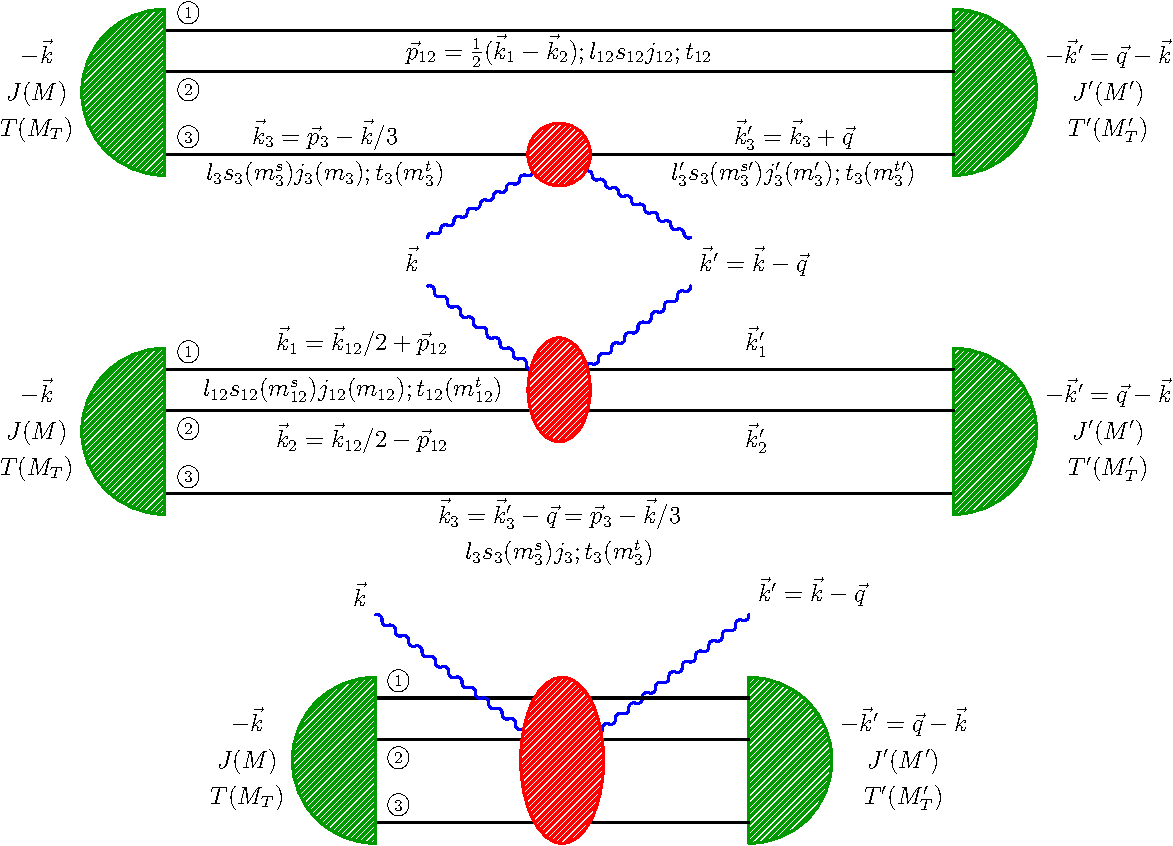
\includegraphics[scale=0.7]{kinematics3He.pdf}
    \caption{Kinematics in the center of mass frame and quantum
      numbers for an $A=3$ system in the case of Compton scattering.
      Generalization to other reactions only changes the
      ingoing/outgoing probe. Generalization to $A>3$ would result in more internal lines
      representing the nucleons.
      Top: one-body processes $\hat{O}_1$ (one active nucleon, two spectators),
      center: two-body
      processes $\hat{O}_{2}$ (two active nucleons, one spectator), bottom: three-body processes
      $\hat{O}_{3}$ (all nucleons active, no spectators). Red represents the kernels; 
      everything else is represented by the densities.
      Green represents the wavefunction of the nucleons.
      $J(M)$ is the spin (projection) and  $T(M_T)$ is the isospin (projection) of the nucleus. 
      $l_i,s_i(m_i^s),j_i(m_i), t_i(m_i^t)$  refer to the angular momentum, spin angular momentum, total angular momentum, isospin (and their projections where appropriate) of the specific subsystem in the kernel being considered.
      From Grie{\ss}hammer \etal
    \cite{hammer2020}.
    \ques{This is getting kind of wordy...}
  }
    \label{fig:onetwobod}
  \end{center}
\end{figure}
For scattering off an $A$-body nucleus, the total scattering
amplitude is given by 
% \begin{align}
%   A_{M}^{M^{\prime} }(\bv{k}, \bv{q})&=\binom{A}{1}\left\langle
%   M^{\prime}\right|\hat{O}_{1}^{}(\bv{k}, \bv{q})\left|M\right
%   \rangle + \binom{A}{2} \left\langle
%   M^{\prime}\right|\hat{O}_{2}^{}(\bv{k}, \bv{q}) \left|
%   M\right\rangle
%   &+... + \binom{A}{A}\left\langle
%   M^{\prime}\right|\hat{O}_{A}^{}(\bv{k}, \bv{q})\left|M\right
%   \rangle
% \end{align}

\begin{align}
  A_{M}^{M^{\prime} }(\bv{k}, \bv{q})&=
 \left\langle M^{\prime}\left|
  \binom{A}{1} \hat{O}_{1}(\bv{k}, \bv{q}) +
  \binom{A}{2} \hat{O}_{2}(\bv{k}, \bv{q}) +... + 
  \binom{A}{A} \hat{O}_{A}(\bv{k}, \bv{q})
  \right|M
  \right\rangle
\end{align}
where $\hat{O}_i$ is the $i$-body kernel, $M,M'$ is the spin projection of the
target nucleus, and there are
$\binom{A}{i}$ ways for a probe to hit $i$ nucleons. 
Fortunately, \ChiEFT provides small dimensionless expansion parameter $\delta\approx 0.4$ \cite{hammer4He} which predicts a
hierarchy of scales for probe energies greater than
$\gtrsim 40 \MeV$ \cite{Griesshammer2012, Hildebrandt2005,Hildebrandt2010}.
Therefore, the 3-body contribution and higher are negligible at this
order, and we simply use
\begin{equation}
  A_{M}^{M^{\prime} }(\bv{k}, \bv{q})=\binom{A}{1}\left\langle
  M^{\prime}\right|\hat{O}_{3}^{}(\bv{k}, \bv{q})\left|M\right
  \rangle + \binom{A}{2} \left\langle
  M^{\prime}\right|\hat{O}_{2}^{}(\bv{k}, \bv{q}) \left|
  M\right\rangle\nonumber\\
\end{equation}
In practice, this is enough for accuracy on roughly the 5\% level \cite{hammer2020}. 
%%%%%%%%%%%%%%%%%%%%%%%%%%%%%%%%%%%%%%%%%%%%%%%%%%%%%%%%%%%%
\section{Kernels and Densities}
The one-body and two-body kernel must be considered separately.
Their form is different, and they require a one- and
two-body density respectively.
Symbolically, the matrix element $\hat{O}_1$ is rather involved and can be found in Griesshammer \etal 
\cite{hammer2020, hammer4He}.
The central result is that up to boost corrections it can
be written as:
\begin{align}
  \left\langle M^{\prime}\left|\hat{O}_{1}(\bv{k}, \bv{q})\right|
  M\right\rangle=\sum_{\substack{m_{3}^{s \prime}\,
  m_{3}^{s}\\m_3^t}}\hat{O}_{1}\left(m_{3}^{s \prime} m_{3}^{s},
  m_{3}^{t} ;  \bv{k}, \bv{q}\right) \rho_{m_{3}^{s \prime}
  m_{3}^{s}}^{m_3^{t} M_{T}, M^{\prime} M}(\bv{k}, \bv{q})\label{onebodyOrig}\;.
\end{align}
Here $\rho$, is the \textit{one-body transition density amplitude} (TDA)
for the nucleus and can be
interpreted as the probability amplitude that nucleon with isospin projection $m_3^t$ absorbs
momentum $\bv{q}$, changes its spin projection from $m_s^3$ to
$m_s^{3'}$ and changes the spin-projection of the nucleus from $M$ to
$M'$, hence the name "Transition Density Amplitude".
Additionally, $M_T$ is the isospin projection of the entire nucleus and $\vec{k}$ is the momentum of the incoming probe.
The two-body case works similarly, and results in
\begin{equation}
  \left\langle M^{\prime}\left|\hat{O}_{2}\right| M\right\rangle =
  \sum_{\alpha_{11}^{\prime}, \alpha_{12}} \int \mathrm{d} p_{12}\:
  p_{12}^{2} \mathrm{~d} p_{12}^{\prime}\: p_{12}^{\prime 2}\;
  \hat{O}_{2}^{\alpha_{12}^{\prime} \alpha_{12}}\left(p_{12}^{\prime},
  p_{12}\right) \rho_{\alpha_{12}^{\prime} \alpha_{12}}^{M_{T},
  M^{\prime} M}\left(p_{12}^{\prime}, p_{12} ; \bv{q}\right)\label{twobody}\;.
\end{equation}
Where 
\begin{equation}
  | \alpha \rangle =|\left[(l_{12}s_{12})j_{12}(l_3 s_3)j_3\right] JM,\;(t_{12}t_3)TM_T\rangle
\end{equation}
This is the two-body equivalent to \eqref{onebodyOrig}.
The two-body density $\rho_{\alpha_{12}^{\prime}
\alpha_{12}}^{M_{T}, M^{\prime} M}$ is of course distinct
from the one-body density.
Moreover, just like the one-body case, it can be interpreted as a
transition probability density amplitude.
It depends on the incoming and outgoing quantum numbers
$\alpha_{12}$ and $\alpha_{12}'$ of the system of the two active nucleons, and also on their initial and final
relative momenta $p_{12}$ and $p_{12}'$ (also of the two nucleons) which are integrated over \com{it's not the 2 nucleons which are integrated over but their rel momenta. Need better formulation!}.\ques{I do not understand what you mean, isn't this what I am already saying?}
As a result, the file size for the two nucleon densities is approximately 20 MB
per energy and angle, whereas those of the one
nucleon densities are on the order of a few KB.
Importantly, the densities $\rho$ can for a given momentum transfer $\vec{q}$ be computed directly from a nuclear
potential, such as the chiral Semilocal Momentum-Space (chiral SMS) potential
\cite{Reinert2018}
without reference to the kernel $\hat{O}_1$ or $\hat{O}_{2}$.
%%%%%%%%%%%%%%%%%%%%%%%%%%%%%%%%%%%%%%%%%%%%%%%%%%%%%%%%%%%%%%%%%%%%%%%
\section{SRG Transformation}
Previous work using the TDA formalism has analyzed
$\HeT$ and $\HeF$
\cite{hammer2020, hammer4He}, but to extend this to $\LiS$ involves more interactions
and as a result the calculation is more complicated and computationally expensive.
To make the calculation of a TDA feasible for $A>6$, a
\textit{Similarity Renormalization Group} (SRG) transformation
is employed \cite{SRG, Furnstahl2013}.
This is of much experimental interest since $\LiS$ is a stable solid at room temperature and is
therefore relatively simple to conduct an experiment on.
There has been some experiments on$\LiS$ \cite{60MeV,86MeV}, yet to date there is no theory prediction.
We seek to fill in this gap.
When using nuclear potentials, we approximate the nucleon-nucleon potential to be zero
beyond a certain cutoff $\LamNN$, and consequently
neglect contributions above this cutoff in our calculations.
In general, a nuclear potential, such as the chiral SMS potential \cite{Reinert2018} does
not fall off rapidly at high momenta.
As a result we would have to
extend the cutoff $\LamNN$ which in turn significantly increases the computational cost.
The SRG transformation is a unitary transformation that
shifts the relevant physics into the low-momentum
region, thereby lowering minimum effective $\LamNN$ in the SRG evolved space.
This, in turn, significantly improves the convergence rate of calculations for $A=6$ making them actually possible.

The SRG transformation can be thought of as a local averaging or
smoothing of the potential, resulting in decreased ``resolution''
as the SRG is applied, however it does this without losing any of the underlying information or compromising the physics.
\begin{figure}[H]
  \centering
  \begin{subfigure}{0.45\textwidth}
    \centering
    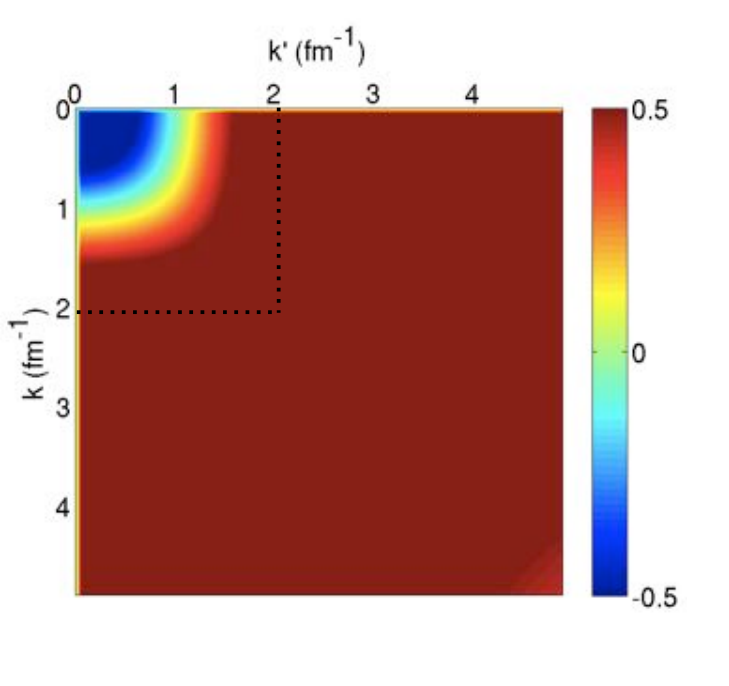
\includegraphics[width=\linewidth]{HighRes.png}
    \caption{High Resolution (before much SRG is applied) }
    \label{fig:highres}
  \end{subfigure}
  \hfill
  \begin{subfigure}{0.45\textwidth}
    \centering
    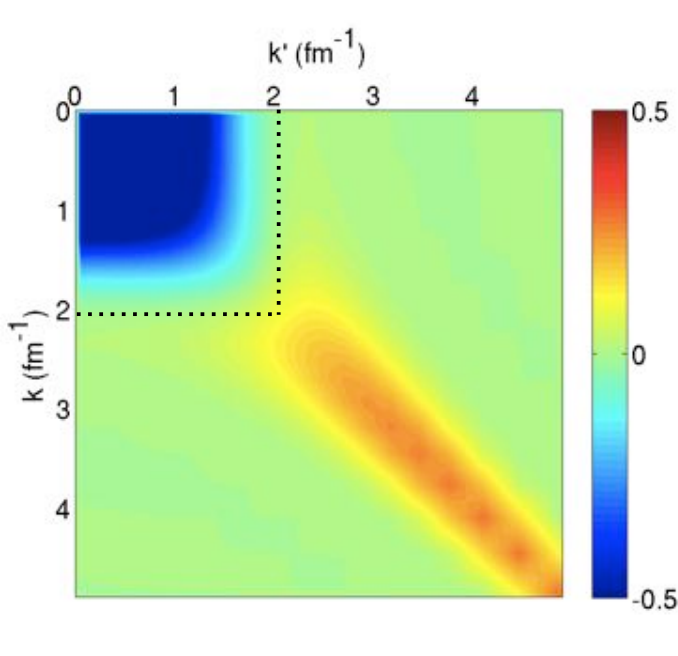
\includegraphics[width=\linewidth]{LowRes.png}
    \caption{Low Resolution (evolved)}
    \label{fig:lowres}
  \end{subfigure}
  \caption{Nuclear potentials $V(k,k')$. Figures from Kai Hebeler:
    ``Chiral Effective Field Theory and Nuclear Forces:
    overview and applications'' presentation at TALENT school at MITP
    2022, and modified with permission from
    Furnstahl \etal \cite{Furnstahl2013}.
  }
  \label{fig:SRGtransform}
\end{figure}
In the under-evolved, high resolution panel, fig.~\ref{fig:highres}, the potential does 
not go to zero rapidly at large momenta, whereas it does once the
transformation is applied in the right panel, fig.~\ref{fig:lowres}. As a
result, a cutoff can be made at $\LamNN=2 \mathrm{fm}^{-1}$ without
losing much accuracy, whereas the under-evolved potential required at least $\LamNN=5 \mathrm{fm}^{-1}$.
The time complexity is at a minimum proportional to the number of array elements
present, therefore we gain at least a factor of $(5/2)^2=6.25$ in efficiency;
in practice the gains are even higher because near-zero values of the potential at large momenta means sparser grids can be used there.

\com{where are you talking about the NCSM as a method to compute 6Li?}\ques{I don't, I didn't feel it was relevant here. We will include it in the next paper.}

The SRG transformation is essential, but it also creates a
change in the physical meaning of the free variables.
In fact, any unitary transformation ($U^\dag U =\mathbbm{1}$) also transforms the coordinates:
\begin{align}
  \br{p'}V\kt{p} 
  = \br{p'} U^\dag U V U^\dag U \kt{p}
  = \br{p'} U^\dag\left( U V U^\dag\right)\;U
  \kt{p}
  = \br{\widetilde{p}\,'} V_{eff}
  \kt{\widetilde{p}}=V_{eff}(\widetilde{p},\widetilde{p}\,')
\end{align}
So referring to the free variables in an SRG-transformed potential as
``momenta'' is, to some extent, incorrect.
They do not represent physical states  in the sense that they are not eigenstates to physical momenta.
The Lagrangeans that generate the Feynman diagrams in the kernel, however,
depend on physical momenta, and therefore we cannot directly use an SRG
evolved potential in the non-SRG evolved kernel.
To solve this, previous work with SRG transformations has transformed the
Lagrangeans - and therefore the kernels - into the SRG evolved space
as well\ques{get citation}.
However, in the context of the density formalism this would mean adding SRG
dependence into the kernel, thereby breaking kernel-density independence. 
This is undesirable since it means more work for the group developing the kernel;
in particular it would mean one would have to transform the kernel with the SRG corresponding to the density every time a 
new SRG evolved density is applied.
Additionally, the SRG transformation can take many different forms \cite{SRG, Furnstahl2013};
we wish to allow for these developments
without having to re-write the kernel code.
Therefore, we developed a method whereby we first perform an SRG, then compute the densities via the SRG evolved potential, and then apply an inverse SRG transformation to the densities \cite{XiangXiang}. 

The process of completing the SRG evolution of the potential, solving for the wavefunction,
and then applying the inverse transformation has parameters that must be fine-tuned, but this
allows for uncertainty estimation.
To solve for the nucleus wavefunction an expansion in the harmonic oscillator basis is used
\ques{I want to avoid referencing the basis used as much as possible. I only do it here because we need to motivate $\omega_H$. It's fine for the next paper, but too much detail here in my opinion}.
When expanded to infinite order, this basis forms a complete set,
however, we truncate this expansion by including harmonic oscillator excitations up to $\Ntot$.
Additionally, the harmonic oscillator basis has a characteristic
width, denoted by $\omega_H$, and finally, the parameter $\LamSRG$
represents the SRG evolution of the potential, as seen in figure
\ref{fig:SRGtransform}. $\LamSRG=\infty$ corresponds to no evolution.
As we will see all of these parameters affect the resulting cross-section. 
We note that above a certain minimum value uncertainty decreases with increasing
$\Ntot$, and at $\Ntot=\infty$ the associated uncertainty goes to zero.

Unfortunately the application of the cutoff in the SRG transformation results in it no longer being strictly unitary. 
Our method neglects the resulting induced many-body  forces, and it is essential to test its impact.
The $\HeF$ system is the highest nucleon number system we can calculate without using the SRG evolution, therefore in order to prepare for $\LiS$ where we cannot preform the raw calculation, we first assess this method's viability on $\HeF$. 
Fortunately figure \ref{fig:SRGConverge4He} shows the uncertainty associated with this approach is small.

During the TDA calculation, we obtain the binding energy of the simulated system, which we can use calibrate our parameters through comparison to the known experimental value.
We determine an optimal $\omega_H$ that yields a good binding energy, while $\Ntot$ is taken as large as feasible.
With this benchmark established, we have extended our analysis to $\LiS$, for which only the SRG evolved form is accessible.
Future investigations \cite{upcoming} will carefully assess the extent to which different $\LamSRG$ values extrapolate to compatible results.


\begin{figure}[H]
  \begin{center}
    \includegraphics[width=\linewidth]{
    4HeCrossSection.rel-dev-SRG-vs-nonSRG.chiralsmsN4LO+3nfN2LO-Λ550.Odelta2.pdf}
    \caption{$\HeF$\, Compton scattering SRG convergence, comparing the exact, vs SRG evolved approaches. Deviations are due to induced manybody forces. ``Relative deviation, (Rel. deviation) of $A$ from $M$''$:= \frac{A}{M}-1$}
    \label{fig:SRGConverge4He}
  \end{center}
\end{figure}
In figure \ref{fig:SRGConverge4He}, we see the effectiveness of the
results in the $\HeF$ case.
We expect the deviation to decrease as $N$ increases, and importantly
for our analysis, this shows what value of $N$ is required.
The small error present at high $\Ntot$ is present do to the induced many body forces.


\begin{figure}[H]
  \centering
  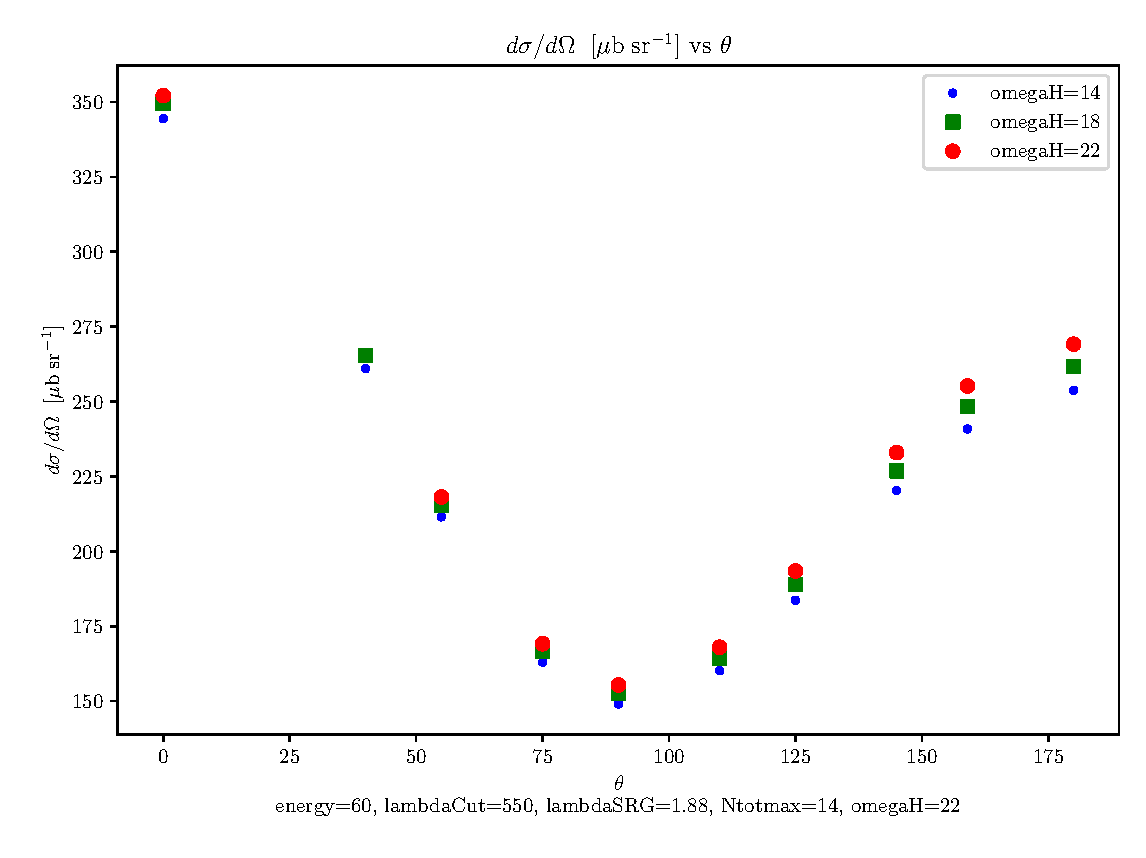
\includegraphics[scale=0.5]{6Li-omegaH-vary.pdf}
  \caption{Caption}
  \label{fig:label1}
\end{figure}

\com{from here on, presentation needs a lot more verbiage and detail -- but I guess you know that}

\com{discuss input: kernels same as in 34He (reference), central values of polarisabilities same as there (aae central values of most recent extractions, reference). Comparison to HIGS data is good/bad/undecided. Will study convergence in detail. Here assumed overall 10\% error as in 34He from potential/cutoff variations plus order-by-order convergence plus numerics plus extrapolations in LambdaSRG/Ntotmax/omegaH,... get inspired by 1-paragraph summary in 4He paper. }

\begin{figure}[H]
  \centering
  %\includegraphics[width=\linewidth]{file_path}
  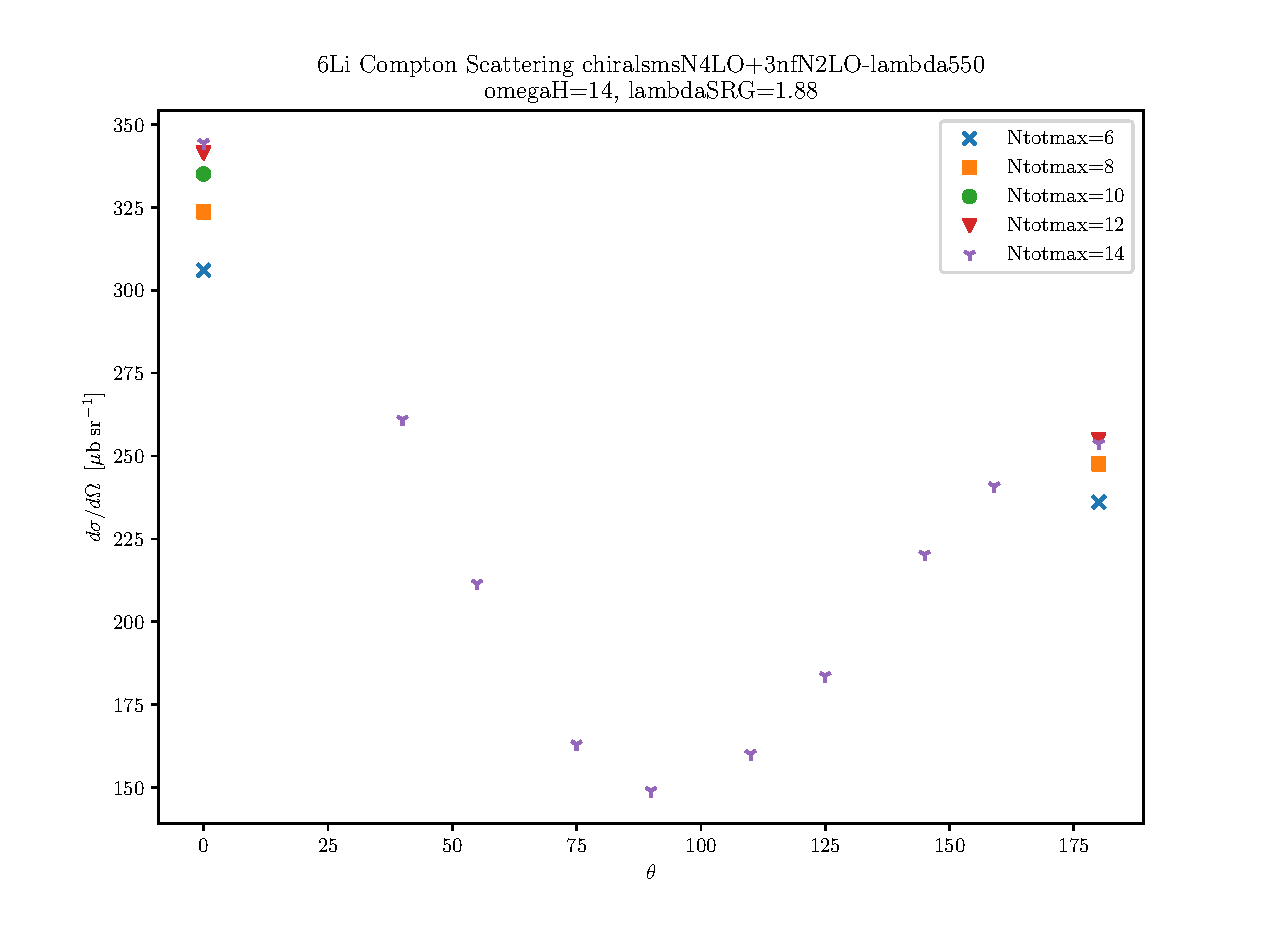
\includegraphics[scale=0.5]{6Li-Ntotmax-vary-omegaH14.pdf}
  \caption{Caption}
  \label{fig:label2}
\end{figure}
%%%%%%%%%%%%%%%%%%%%%%%%%%%%%%%%%%%%%%%%%%%%%%%%%%%%%%%%%%%%%%%%%%%%%
\section{Using TDAs in different processes}
With the TDAs calculated for Compton scattering, we now wish to recycle them for new processes.
In particular pion-photoproduction, and
pion scattering are of interest.
Fortunately their kernels share remarkable similarity since if one ignores the type of incoming/outgoing 
particle the processes are topologically identical.
\begin{figure}[H]
\centering
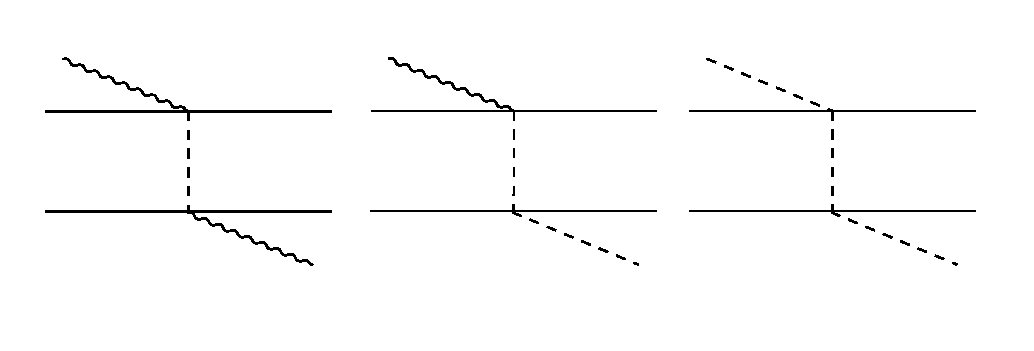
\includegraphics[scale=0.5]{KernelSim.pdf}
\caption{Topologically identical diagrams in Compton scattering, pion-photoproduction, and pion scattering \com{twobody only -- add onebody?}\ques{I'd rather not}}
\end{figure}
\subsection{Pion-Photoproduction}
For the pion-photoproduction one-body kernel, we use the results from
single-nucleon scattering, $\gamma N \to \pi N$ which has
been studied extensively both in \ChiEFT and phenomenologically \cite{pionphoto,
Rijneveen2021,Workman2012,Briscoe2023}.
Its differential cross section can be decomposed into the
electric and magnetic multipoles $E_{l\pm}, M_{l\pm}$ \cite{pionphoto}.
Over the years, many experiments have measured
these multipoles to high order and with good precision
\cite{multipolePionPion}.
The resulting scattering matrices $\mathcal{M}$ are exactly what
enters as $\hat{O}_1$ in equation (\ref{onebodyOrig}).
This approach solves a significant problem since the calculation of
the one-body pion-photoproduction kernel
to high accuracy directly from Feynman diagrams requires including many terms
in the chiral expansion due to the proximity of the $\Delta(1232)$ resonance at $\sim 200\MeV$.
A theoretical prediction of these multipoles is given by Rijneeven et al \cite{Rijneveen2021}, which we intend to compare 
to experimental data.


The two-body contributions do not easily decompose into multipoles, so we perform the calculation through expansions
in the chiral Lagrangean via calculation of Feynman diagrams.
To this end Beane \etal $\cite{Beanephotoprod}$ provides the kernel for the reaction on the deuteron at threshold
and since we only go up to the two-body kernel this is sufficient for our needs.
Additionally this reaction kernel has been analyzed by
Lenkewitz \etal \cite{L2011, L2013} who considers the targets $\HeT$ and $\HThree$.
We now have a numerically stable result for $\HeT$ and seek to extend
this approach to new targets.
\ques{Include some numbers, need to discuss with you uncertainty analysis.} \com{yes!!!!}


\subsection{Pion scattering and other reactions}
Beane \etal have developed the pion scattering kernel at threshold for both
one-body and two-body interactions \cite{Beane2003}.
We anticipate extending this analysis to finite energy the targets $\HThree, \HeT, \HeF, \LiS$
Once the pion-photoproduction and pion-pion scattering kernels have
successfully been developed, we will be able to calculate all of
these reactions on previously analyzed targets in the density
formalism since we already have produced most of the TDAs required.
In particular, we will calculate all of these reactions with the
targets $\HThree$, $\HeT$, $\HeF$, and $\LiS$. \com{relocate to 2 sentences prior}

\com{why is this interesting? first study (?) of ChiSym in these processes at heavier nucei. But beware Braun PhD thesis: maybe cite to reflect literature?}

%%%%%%%%%%%%%%%%%%%%%%%%%%%%%%%%%%%%%%%%%%%%%%%%%%%%%%%%%%%%%%%%%%%%%%%%%%%%%%%%%%%%%%
\section{Conclusion}
We have described a comprehensive framework for
computing scattering observables in light nuclei by factorizing the
full amplitude into target‐dependent few-body transition density
amplitudes (TDAs) and probe‐dependent interaction kernels. 
This work expands on work in refs, as well as work on few body targets \cite{hammer2020,hammer4He,L2013}.
This separation allows us to treat the nuclear structure and the
reaction mechanism independently, thereby streamlining the
calculation of observables.
The central thrust of this work is the successful extension of
the density formalism to heavier targets like $\LiS$ by incorporating a
similarity renormalization group (SRG) transformation.
The SRG not only accelerates the convergence of our calculations by
lowering the effective momentum cutoff, but—when combined with an
appropriate inverse transformation of the densities—also preserves
the kernel–density independence that is crucial for the versatility
of our approach.
Furthermore, we have presented preliminary results for Compton scattering on
% \com{you could write sth like "we presented first and preliminary results on.... Compton 6Li, summarising some key findings of an upcoming publication \cite{} which will also address pols sensitivity, detailed convergence study, detailed study of numerical and theory uncertainties, of world peace,...}
$\LiS$ which agrees
\ques{check this}
agrees well with data, and we have outlined the ongoing extension of the formalism to other
reactions, such as pion-photoproduction and pion scattering on light nuceli\cite{upcoming} \ques{You have a note saying to I cite my proposal, but how? We never published it.}  %\cite{cite your thesis proposal and upcoming publication!}.
The ability to plug in different reaction kernels into the same TDA
framework and vice versa not only enhances the predictive power of our approach but
also paves the way for a unified treatment of various scattering
processes in a wide range of few-body systems.
Ultimately, this framework provides a promising route toward
high-precision theoretical predictions, deepening our understanding
of nuclear dynamics in light nuclei.

%%%%%%%%%%%%%%%%%%%%%%%%%%%%%%%%%%%%%%%%%%%%%%%%%%%%%%%%%%%%%%%%%%%%%%%%%%%%%%%%%%%%%%
\section{Acknowledgements}
\com{acknowledgments: Andreas+, supercomputer usage, DOE and DFG grants -- see 4He paper}
We thank Andreas Nogga and Xiang-Xiang Sun of FZ J{\"u}lich, whos' work on produces the required TDAs we 
deeply appreciate.
\ques{Below is a copy paste of all of the acknowledgements from 4He that might be relevant, this 
obviously needs to be fixed for this paper
}

We appreciate the warm hospitality and
financial support for stays which were instrumental for this research: HWG at the University
of Manchester, Ohio University and FZ J¨ulich; and DRP at George Washington University
and Chalmers University of Technology. HWG is grateful to the organisers and participants
of the meeting of MAMI’s A2 collaboration in Mainz for the stimulating atmosphere and
financial support. He also thanks the organisers and participants of MENU 2023 in Mainz
for the opportunity to present preliminary results and for a delightful atmosphere. This
work was supported in part by the US Department of Energy under contract DE-SC0015393
(HWG, JL) and DE-FG02-93ER-40756 (DRP), by the UK Science and Technology Facilities
Council grant ST/P004423/1 (JMcG), by the Deutsche Forschungsgemeinschaft and the
Chinese National Natural Science Foundation through funds provided to the Sino-German
CRC 110 “Symmetries and the Emergence of Structure in QCD” (AN; DFG grant TRR 110;
NSFC grant 11621131001), by the Ministerium f¨ur Kultur und Wissenschaft NordrheinWestphalen (MKW-NW) under funding code NW21-024-A (AN) and by a Tage Erlander
Professorship from the Swedish Research Council, grant 2022-00215 (DRP). Additional
funds for HWG were provided by an award of the High Intensity Gamma-Ray Source HI$\gamma$S
of the Triangle Universities Nuclear Laboratory TUNL in concert with the Department of
Physics of Duke University, and by George Washington University: by the Office of the
Vice President for Research and the Dean of the Columbian College of Arts and Sciences;
by an Enhanced Faculty Travel Award of the Columbian College of Arts and Sciences.
His research was conducted in part in GW’s Campus in the Closet. The computations of
nuclear densities were performed on Jureca of the J{\"u}lich Supercomputing Centre (J¨ulich,
Germany).

%%%%%%%%%%%%%%%%%%%%%%%%%%%%%%%%%%%%%%%%%%%%%%%%%%%%%%%%%%%%%%%%%%%%%%%%%%%%%%%%%%%%%%
\begin{thebibliography}{99}
  \bibitem{hammer2020}
  H. W. Grie{\ss}hammer, J. A. McGovern, A. Nogga, and D. R.
  Phillips, ``Scattering Observables from One- and Two-body
  Densities: Formalism and Application to $\gamma^3$ Scattering,''
  \textit{Few-Body Systems}, vol. 61, no. 4, Nov. 2020. DOI:
  \href{https://doi.org/10.1007/s00601-020-01578-w}{10.1007/s00601-020-01578-w}.

  \bibitem{Reinert2018}
  P. Reinert, H. Krebs, and E. Epelbaum, ``Semilocal momentum-space
  regularized chiral two-nucleon potentials up to fifth order,''
  \textit{The European Physical Journal A}, vol. 54, no. 5, May 2018.
  DOI:
  \href{http://dx.doi.org/10.1140/epja/i2018-12516-4}{10.1140/epja/i2018-12516-4}.
  \bibitem{hammer4He}
Grießhammer, H.W., Liao, J., McGovern, J.A. et al. Compton scattering on 
 with nuclear one- and two-body densities. Eur. Phys. J. A 60, 132 (2024). https://doi.org/10.1140/epja/s10050-024-01339-x
\href{https://arxiv.org/abs/2401.16995}{arXiv:2401.16995}.

\bibitem{SRG}
S. Szpigel and R. J. Perry, ``The Similarity Renormalization Group,'', Quantum Field Theory: A Twentieth Century Profile,
Sep. 2000. \href{https://doi.org/10.48550/arXiv.hep-ph/0009071}{https://doi.org/10.48550/arXiv.hep-ph/0009071}

\bibitem{pionphoto}
R. L. Walker, ``Phenomenological Analysis of Single-Pion
Photoproduction,'' \textit{Phys. Rev.}, vol. 182, no. 5, pp.
1729--1748, Jun. 1969. DOI:
\href{https://link.aps.org/doi/10.1103/PhysRev.182.1729}{10.1103/PhysRev.182.1729}.

\bibitem{multipolePionPion}
R. L. Workman, M. W. Paris, W. J. Briscoe, and I. I. Strakovsky,
``Unified Chew-Mandelstam SAID analysis of pion photoproduction
data,'' \textit{Phys. Rev. C}, vol. 86, no. 1, p. 015202, Jul.
2012. DOI:
\href{https://link.aps.org/doi/10.1103/PhysRevC.86.015202}{10.1103/PhysRevC.86.015202}.

\bibitem{Rijneveen2021}
N. Rijneveen, A. M. Gasparyan, H. Krebs, and E. Epelbaum, ``Pion photoproduction in chiral perturbation theory with explicit treatment of the $\Delta(1232)$ resonance,'' \textit{Phys. Rev. C}, vol. 106, no. 2, p. 025202, Aug. 2022. DOI: \href{https://link.aps.org/doi/10.1103/PhysRevC.106.025202}{10.1103/PhysRevC.106.025202}.

\bibitem{L2011}
M. Lenkewitz, E. Epelbaum, H.-W. Hammer, and U.-G. Meißner,
``Neutral pion photoproduction off $^3$H and $^3$He in chiral
perturbation theory,'' \textit{Physics Letters B}, vol. 700, no. 5,
pp. 365–368, Jun. 2011. DOI:
\href{http://dx.doi.org/10.1016/j.physletb.2011.05.036}{10.1016/j.physletb.2011.05.036}.

\bibitem{L2013}
M. Lenkewitz, E. Epelbaum, H.-W. Hammer, and U.-G. Meissner,
``Threshold neutral pion photoproduction off the tri-nucleon to
$O(q^4)$,'' \textit{The European Physical Journal A}, vol. 49, no.
2, Feb. 2013. DOI:
\href{http://dx.doi.org/10.1140/epja/i2013-13020-1}{10.1140/epja/i2013-13020-1}.

\bibitem{86MeV}
L. S. Myers, M. W. Ahmed, G. Feldman, A. Kafkarkou, D. P.
Kendellen, I. Mazumdar, J. M. Mueller, M. H. Sikora, H. R. Weller,
and W. R. Zimmerman, ``Compton scattering from $^{6}\mathrm{Li}$ at
86 MeV,'' \textit{Phys. Rev. C}, vol. 90, no. 2, p. 027603, Aug.
2014. DOI:
\href{https://link.aps.org/doi/10.1103/PhysRevC.90.027603}{10.1103/PhysRevC.90.027603}.

\bibitem{60MeV}
L. S. Myers, M. W. Ahmed, G. Feldman, S. S. Henshaw, M. A. Kovash,
J. M. Mueller, and H. R. Weller, ``Compton scattering from $^{6}$Li
at 60 MeV,'' \textit{Phys. Rev. C}, vol. 86, no. 4, p. 044614, Oct.
2012. DOI:
\href{https://link.aps.org/doi/10.1103/PhysRevC.86.044614}{10.1103/PhysRevC.86.044614}.

\bibitem{Beane2003}
S. R. Beane, V. Bernard, E. Epelbaum, U.-G. Meißner, and D. R.
Phillips, ``The S-wave pion–nucleon scattering lengths from pionic
atoms using effective field theory,'' \textit{Nuclear Physics A},
vol. 720, no. 3–4, pp. 399–415, Jun. 2003. DOI:
\href{http://dx.doi.org/10.1016/S0375-9474(03)01008-X}{10.1016/S0375-9474(03)01008-X}.

\bibitem{Workman2012}
R. L. Workman, M. W. Paris, W. J. Briscoe, and I. I. Strakovsky,
``Unified Chew-Mandelstam SAID analysis of pion photoproduction
data,'' \textit{Phys. Rev. C}, vol. 86, no. 1, p. 015202, Jul.
2012. DOI:
\href{https://link.aps.org/doi/10.1103/PhysRevC.86.015202}{10.1103/PhysRevC.86.015202}.
\bibitem{Briscoe2023}
W. J. Briscoe, A. Schmidt, I. Strakovsky, R. L. Workman, and A.
\ifmmode \check{S}\else \v{S}\fi{}varc, ``Extended SAID
partial-wave analysis of pion photoproduction,'' \textit{Phys. Rev.
C}, vol. 108, no. 6, p. 065205, Dec. 2023. DOI:
\href{https://link.aps.org/doi/10.1103/PhysRevC.108.065205}{10.1103/PhysRevC.108.065205}.
\bibitem{Furnstahl2013}
R. J. Furnstahl and K. Hebeler, ``New applications of
renormalization group methods in nuclear physics,'' \textit{Reports
on Progress in Physics}, vol. 76, no. 12, p. 126301, Nov. 2013.
DOI:
\href{http://dx.doi.org/10.1088/0034-4885/76/12/126301}{10.1088/0034-4885/76/12/126301}.
\bibitem{XiangXiang}
X.-X. Sun, H. Le, A. Nogga, and U.-G. Meißner, in preparation (2025).

\bibitem{Vries2024}
J. de Vries, C. Körber, A. Nogga, et al., ``Dark matter scattering
off He in chiral effective field theory,'' \textit{Eur. Phys. J.
C}, vol. 84, p. 1138, 2024. DOI:
\href{https://doi.org/10.1140/epjc/s10052-024-13477-z}{10.1140/epjc/s10052-024-13477-z}.

\bibitem{upcoming}
Alexander Long, Harald W. Grie{\ss}hammer, X.-X. Sun, H. Le, A. Nogga,  in preparation (2025).

\bibitem{Griesshammer2012}
H. W. Grie{\ss}hammer, J. A. McGovern, D. R. Phillips, and G. Feldman, ``Using Effective Field Theory to analyse low-energy Compton scattering data from protons and light nuclei,'' \textit{Progress in Particle and Nuclear Physics}, vol. 67, no. 4, pp. 841–897, Oct. 2012. DOI: \href{http://dx.doi.org/10.1016/j.ppnp.2012.04.003}{10.1016/j.ppnp.2012.04}.

\bibitem{Hildebrandt2005}
R. P. Hildebrandt, ``Elastic Compton Scattering from the Nucleon and Deuteron,'' 2005. Available: \href{https://arxiv.org/abs/nucl-th/0512064}{arXiv:nucl-th/0512064}.

\bibitem{Hildebrandt2010}
R. P. Hildebrandt, H. W. Grießhammer, and T. R. Hemmert, ``Nucleon polarizabilities from deuteron Compton scattering within a Green’s function hybrid approach,'' \textit{The European Physical Journal A}, vol. 46, no. 1, pp. 111–137, Sep. 2010. DOI: \href{http://dx.doi.org/10.1140/epja/i2010-11024-y}{10.1140/epja/i2010-11024-y}.
\bibitem{Beanephotoprod}
S. R. Beane, V. Bernard, T.-S. H. Lee, U.-G. Meißner, and U. van Kolck, ``Neutral pion photoproduction on deuterium in baryon chiral perturbation theory to order $q^4$,'' \textit{Nuclear Physics A}, vol. 618, no. 4, pp. 381–401, Jun. 1997. DOI: \href{http://dx.doi.org/10.1016/S0375-9474(97)00133-4}{10.1016/S0375-9474(97)00133-4}.
\end{thebibliography}

\end{document}

